
\chapter{Progetto Logico}
In questo capitolo viene fornita una panoramica generale sul funzionamento del progetto e del comportamento delle sue parti principali. Inoltre viene data un introduzione sull'estensibilità e la personalizzazione sia dell'interprete che della configurazione della scheda FPGA. 

\vspace{0.2cm}

\begin{figure}[h!]
    \centering
    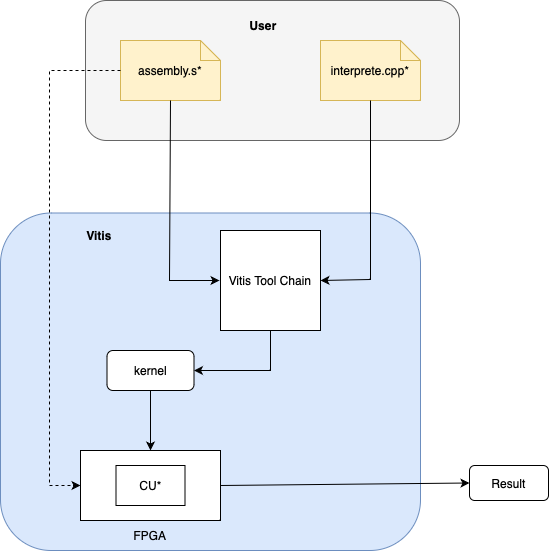
\includegraphics[scale=0.6]{images/Capitolo3/5_im.png}
    \caption{Schema Generale}
    \label{Graficogenerale}
\end{figure}

\clearpage

Come si può osservare dal grafico \ref{Graficogenerale}, il progetto si basa sull'utilizzo un interprete scritto in un linguaggio di alto livello. Questo interprete attraverso la toolchain di Vitis viene trasformato in un kernel eseguibile all'interno dell'FPGA, di cui possono essere istanziate diverse copie (Control Unit), al fine di eseguire programmi anche diversi tra loro.

\vspace{1cm}

Insieme alla configurazione dell'interprete è necessario fornire un file scritto nel linguaggio assembly usato dall'interprete, il quale contiene le istruzioni che saranno eseguite dall'acceleratore, ovvero il programma da eseguire sul softcore. Durante l'esecuzione del Kernel, queste istruzioni presenti nel file assembler vengono caricate nella memoria allocata per il softcore sulla FPGA.

Dopo aver eseguito i calcoli sulla FPGA si otterranno i risultati desiderati. Questi risultati saranno estratti dalla memoria del softcore nella FPGA, e successivamente si potranno osservare nella memoria della macchina host.

\vspace{1cm}

Come si può notare dal grafico, questo progetto offre una grande possibilità di configurazione, con la capacità di effettuare modifiche nelle seguenti aree: 

\begin{itemize}
    \item \textbf{Interprete}: essendo un interprete scritto in linguaggio di alto livello, offre un alto grado di personalizzazione. È possibile specializzarlo scegliendo solo il set di istruzioni più adatto per l'applicazione specifica, oppure estenderlo per interpretare un insieme più grande di istruzioni assembly, o persino cambiare totalmente l'architettura interpretata.
    \item \textbf{Control Unit}: durante il processo della compilazione del kernel, è possibile scegliere quante istanze (CU) allocare all'interno della FPGA. Questo, permette di avere più "core logici" all'interno della scheda FPGA, da gestire in base alle esigenze dell'applicazione.
    \item \textbf{Assembly.s}: questo file, a patto che rispetti il set di istruzioni dell'interprete sviluppato, offre un grande libertà nella scrittura del codice, può contenere qualsiasi flusso di istruzioni consentito dall'interprete. Inoltre è possibile usare file assembly diversi per ciascuna delle CU, cosi da aver più core che eseguono flussi di istruzioni diverse. 
\end{itemize}

\vspace{1cm}

Inoltre (come vedremo nel capitolo Implementazione, Cap. \ref{implementazione}), l'interprete funziona con una memoria dati, e una memoria per i registri, le quali sono altamente anch'esse configurabili in modo da poter soddisfare esigenze diverse.

\clearpage

\section{Funzionamento}
\label{funzionamento}

\noindent Di seguito un grafico sul funzionamento generale delle componenti del progetto.

\begin{figure}[h!]
    \centering
    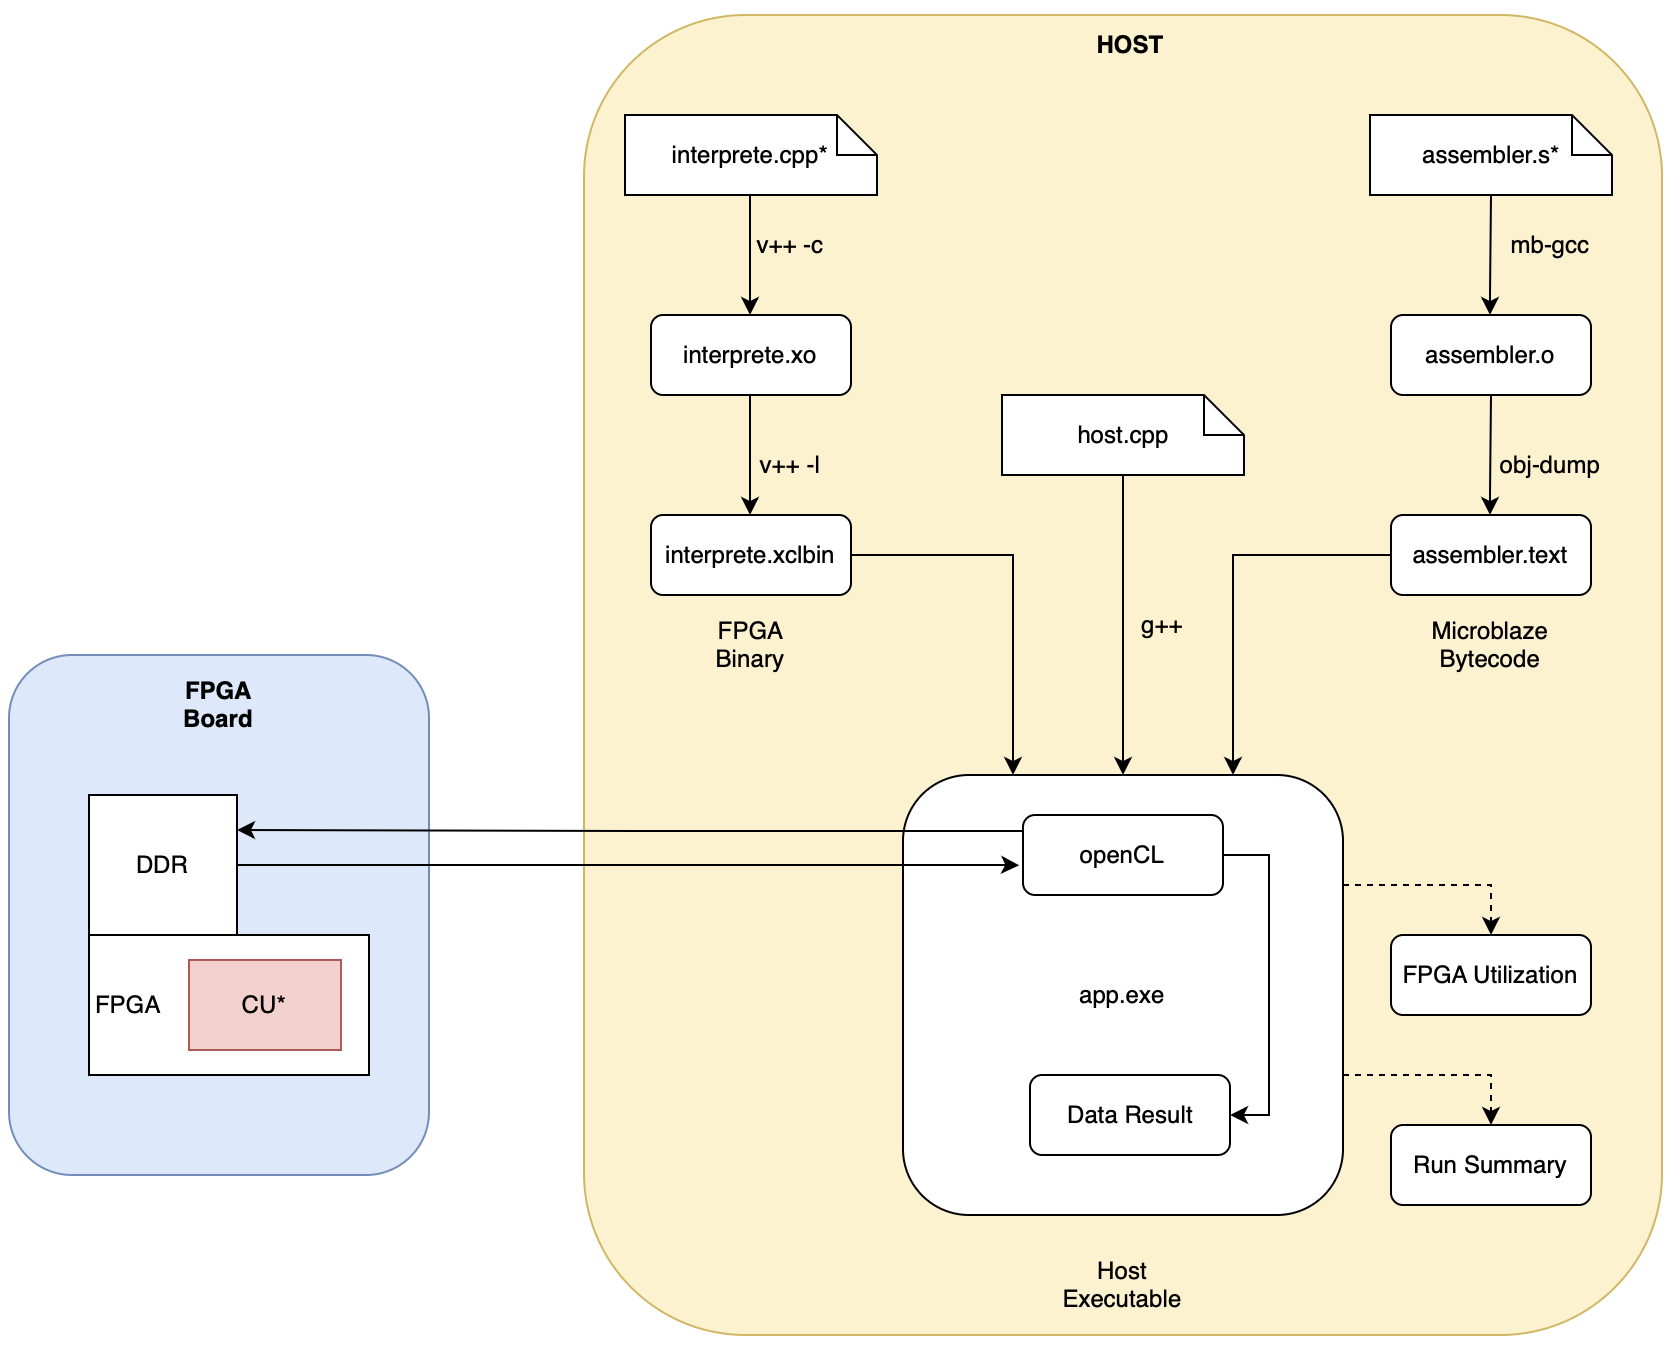
\includegraphics[scale=0.5]{images/Capitolo3/6_im.png}
    \caption{Grafico Funzionamento}
    \label{funzionamentoOpenCL}
\end{figure}

Nel lato hardware del progetto, l'attività si svolge su una macchina host dove in cui è installata la scheda FPGA (la FPGA Board a sinistra in fig. \ref{funzionamentoOpenCL}). Le componenti software del progetto (a sinistra in fig. \ref{funzionamentoOpenCL}) sono suddivise principalmente in tre parti:

\begin{itemize}
    \item \textbf{FPGA Binary}, questo file contiene il Bit Stream FPGA, il quale è l'implementazione hardware del kernel definito nel file \texttt{interprete.cpp}, questo kernel verrà eseguito successivamente dal chip della scheda FPGA.
    \item \textbf{Microblaze Bytecode}, il file contenente il bytecode generato dal compilatore \texttt{mb-gcc}, utilizzando le istruzioni scritte in linguaggio assembly Microblaze, il quale sarà interpretato dal kernel presente nella FPGA.
    \item \textbf{Host Executable}, questo eseguibile compilato tramite \texttt{g++}, viene eseguito sulla macchina host, ed è responsabile di effettuare le chiamate API di OpenCL, istanziare e caricare i dati nella memoria dell'FPGA (DDR), e gestire i risultati ottenuti dall'interpretazione delle istruzioni assembly.
\end{itemize}

\begin{figure}[h!]
    \centering
    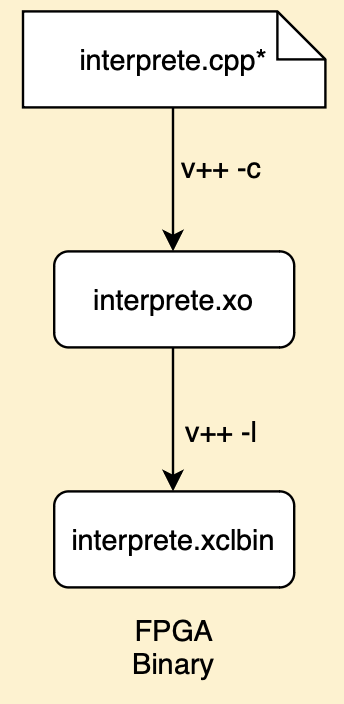
\includegraphics[scale=0.5]{images/Capitolo3/2_im.png}
    \caption{Flusso di Compilazione Interprete}
    \label{funzionamentoOpenCL}
\end{figure}

\noindent Per la generazione del Bit Stream, partiamo da un file chiamato \textbf{interprete.cpp}, dove è definita la funzione principale che verrà eseguita nella scheda FPGA.

All'interno di questo kernel è implementato l'intero interprete del processore Microblaze, il quale legge i dati dalla memoria globale della FPGA, ovvero la memoria dati, la memoria delle istruzioni da interpretare (precedentemente caricate dalla parte host), e la memoria dei registri.
L'Interprete successivamente esegue le istruzioni e trasferisce la sua memoria dati nuovamente nella memoria globale della FPGA.

La creazione di questo file inizia da un file con all'interno una funzione \texttt{extern C}, il quale viene compilato tramite il compilatore fornito dalla toolchain di Vitis chiamato \texttt{v++}, con l'aggiunta della flag \texttt{-c}, la quale specifica di per compilare il codice sorgente in un file \texttt{.xo}, il quale contiene tutti i dati necessari per la successiva generazione del bitstream. Notare che questo processo, che traduce il codice di alto livello del kernel nel linguaggio RTL, richiede un tempo dell'ordine dei minuti o anche secondi, quindi relativamente breve.

Successivamente si compila usando nuovamente \texttt{v++} utilizzando la flag \texttt{-l}, cosi da effettuare il linking del kernel compilato dal file \texttt{.xo}, con la piattaforma target, in modo da generare il bitstream che è contenuto nel file \texttt{.xclbin}, che contiene tutti i dati necessari per configurare l'FPGA con un kernel che implementa l'interprete. È da notare che la durata di questa fase può variare da minuti a ore, in base alla complessità e alla quantità di codice coinvolto. La durata di questo passaggio può variare da minuti a ore di tempo, a seconda della complessità e quantità di codice.


\clearpage

\begin{figure}[h!]
    \centering
    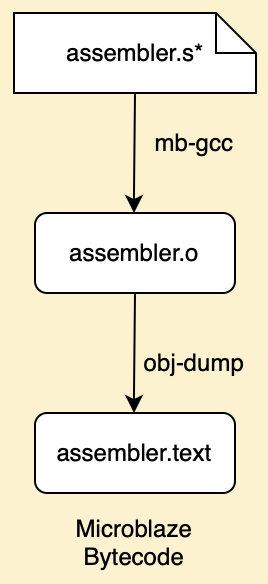
\includegraphics[scale=0.6]{images/Capitolo3/3_im.png}
    \caption{Flusso Assembler}
    \label{flussoassembler}
\end{figure}

\noindent Per la creazione del bytecode si inizia partendo da un file scritto in linguaggio assembly (vedi fig. \ref{flussoassembler}). 

Successivamente usando il compilatore fornito dalla toolchain di Xilinx chiamato \texttt{mb-gcc}, questo file viene compilato in un file "oggetto" \texttt{.o} . Questo file contiene il risultato della compilazione insieme ad altri meta dati aggiunti dal compilatore stesso.

Successivamente tramite l'utilizzo del tool chiamato \texttt{obj-dump} estraiamo la parte \texttt{.text} dal file. Questa sezione contiene le istruzioni assembly tradotte dal compilatore e convertite in uno stream di byte.

\begin{figure}[h!]
    \centering
    
\includegraphics[scale=0.35]{images/Capitolo3/4_im.png}
    \caption{Flusso Host}
    \label{flussohost}
\end{figure}

\noindent Un'ultima parte del progetto riguarda la compilazione dell'eseguibile che sarà eseguito sulla CPU della macchina host (vedi fig.\ref{flussohost}). Questo file svolge un ruolo cruciale nella gestione della FPGA, compresa l'inizializzazione della memoria esterna dove verranno presi i dati, che includono i registri, la memoria dati e memoria delle istruzioni. 

L'eseguibile è responsabile inoltre di caricare (tramite OpenCL) i kernel precedentemente compilati all'interno della scheda FPGA e successivamente di avviare il processo di esecuzione dell'interprete e verifica i risultati ottenuti dall'elaborazione. 
